\chapter{Einführung in den Versuch}
\label{cha:einfuehrung}
\todo{}
\section{Einleitung \(Menzel\)}

Die Im Rahmen dieses Projekts zu behandelnde Aufgabe ist der Aufbau eines Netzwerks aus Sensoren.
Während des HT2024 und des WT2025 hat sich unsere Gruppe mindestens einmal wöchentlich getroffen.
Das Projekt umfasste sowohl die Planung, als auch die Durchführung und Auswertung von Messaufbauten und Versuchen.
Als Grundlage diente ein bereits bestehender Versuchsaufbau an einem Fahrrad, siehe Kapitel \ref{sec:technikstandfahrrad}.
Da im Laufe des Projekts in verschiedenen Entwicklungsteams gearbeitet wurde und jede Gruppe eigenständig an ihren Berichten arbeitete kann es zu Doppelungen im Bericht kommen.

\section{Zielsetzung \(Menzel\)}
Ein Ziel des Projekts ist es, den bestehenden Aufbau am Fahrrad weiterzuentwickeln und zu verbessern.
Hierbei soll die neu entwickelte Technik angewendet werden und vom alten Aufbau sollen lediglich die bereits am Fahrradlenker angebrachten Dehnungsmessstreifen verwendet werden.

Ein weiteres Ziel ist es, an einem anderen Aufbau Sensoren anzubringen.
Dieser andere Aufbau stellt den von LandurisStudio \footcite{https://www.landuris.com/} entwickelten Flying Suit dar.
LandurisStudio ist ein Münchener Startup Unternehmen welches sich mit innovativen Designlösungen in den Bereichen Innenarchitektur, Kunst und Produktdesign befasst.
Besonders zeichnet LandurisStudio die unkonventionelle und künstlerische Herangehensweise aus.


\newpage
\section{Aufgabenverteilung \(Menzel\)}
Um dem Umfang des Projekts gerecht zu werden war es nötig sich zunächst über die Aufgaben bewusst zu werden.
Hierfür wurden diese in einem Projektstrukturplan zusammengefasst. Dies war zunächst eine Herausforderung, da alle am Projekt beteiligten Studenten im Bachelor Technische Informatik und Kommunikationstechnik studiert hatten,
und demnach mit der Herangehensweise eines solchen Aufbaus nicht vertraut waren und sich erst einarbeiten mussten.
Im Laufe des Projekts haben sich einzelne Aspekte des Plans verändert beziehungsweise konkretisiert, dennoch diente der ursprüngliche Entwurf des Plans als grobe Orientierung stets einen Überblick zu haben.
Hier wurde bereits bedacht, dass in der Endphase des Projekts auch noch Zeit für die Erstellung der Präsentation und des Berichts genommen werden muss.

\begin{figure}[h]
    \begin{center}
        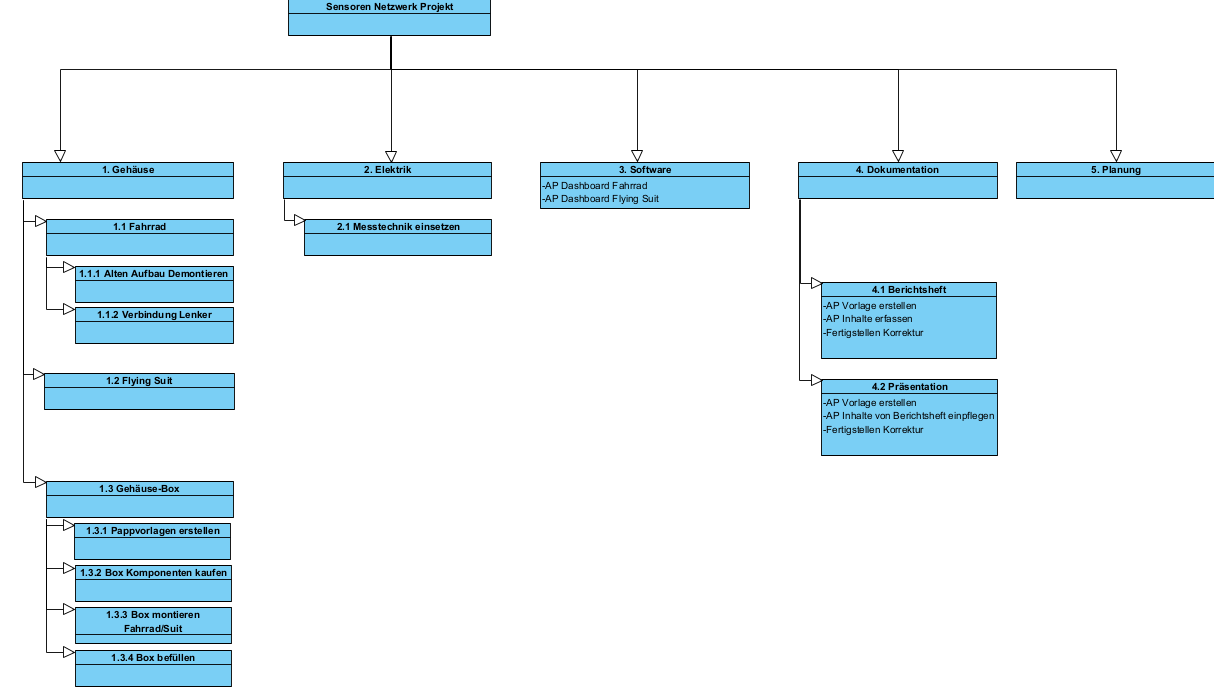
\includegraphics[width=1.0\textwidth, keepaspectratio]{plan.png}
        \caption[Aufgaben (Abbildungsverzeichnis)]{Aufgaben
        %\cite{VLInkManual}
        }
        \label{fig:plan}
    \end{center}
\end{figure}


Aufgrund der Gruppenstärke von fünf Studenten erschien es sinnvoll zunächst eine Aufgabenverteilung und Aufteilung in Teams durchzuführen.
Nachdem sich jeder mit der Aufgabenstellung und den notwendigen theoretischen Grundlagen vertraut gemacht hatte geschah die Aufteilung in die Teams Fahrrad (Bellgardt, Menzel) und Flying Suit (Grote, Nerb, Ulit).
Zu einem späteren Zeitpunkt hat sich vom Team Flying Suit das Team Software (Grote) abgespaltet, siehe Abbildung \ref{fig:aufgabenverteilung}.

Diese Aufteilungen waren sinnvoll, um dem großen Umfang des Projekts gerecht werden zu können. Hierbei hat das Team Fahrrad in den Laboren von Professor Kuttner gearbeitet während das Team Flying Suit einen Großteil ihrer Arbeiten, insbesondere die der Messungen bei Herrn Landuris in dessen Räumlichkeiten durchgeführt haben.

Um erarbeitete Konzepte, Lösungen u.ä. zwischen und innerhalb der Teams nutzen zu können wurde während des Projekts auf TeamDrive zugegriffen um Dateien zugänglich zu machen.
Zur Präsentation des Projekts im Hörsaalrahmen wurde eine geteilte Powerpoint verwendet. Dieser Bericht wurde in Latex erstellt.

\begin{figure}[h]
    \begin{center}
        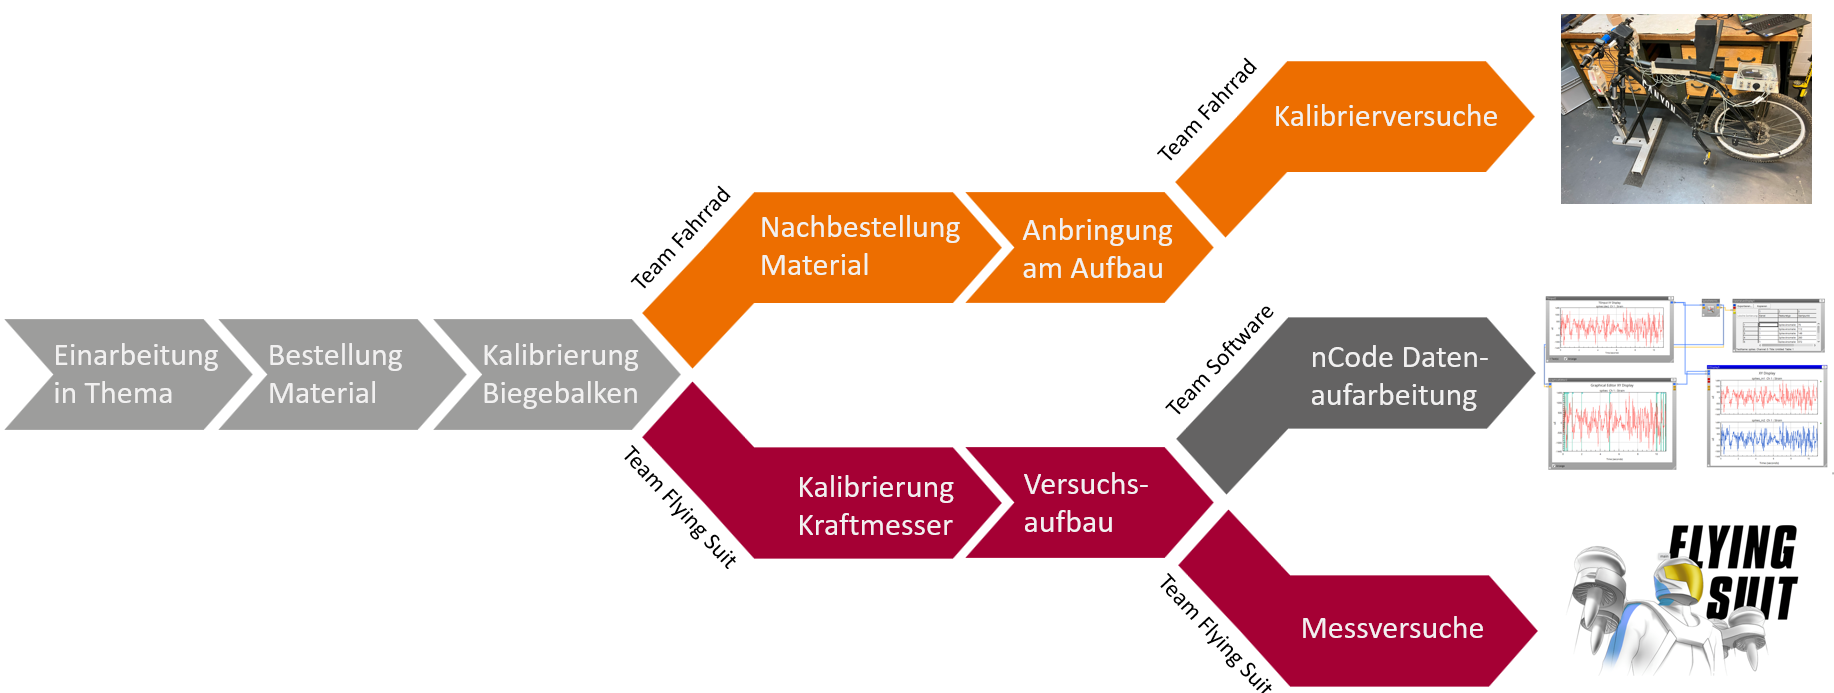
\includegraphics[width=1\textwidth, keepaspectratio]{aufgabenverteilung.png}
        \caption[Aufgabenverteilung Entwicklungsteams (Abbildungsverzeichnis)]{Aufgabenverteilung Entwicklungsteams
        %\cite{VLInkManual}
        }
        \label{fig:aufgabenverteilung}
    \end{center}
\end{figure}